Data preprocessing involved the parsing of the requisite information made available through the dataset; for each student, all courses are paired with their terms of enrollment. In order to preserve the normal, sequential nature of courses across academic years, we omit the Summer Period from all experiments. 
\section{Methodology}
\label{sec:methodology}

\begin{figure}
    \centering
    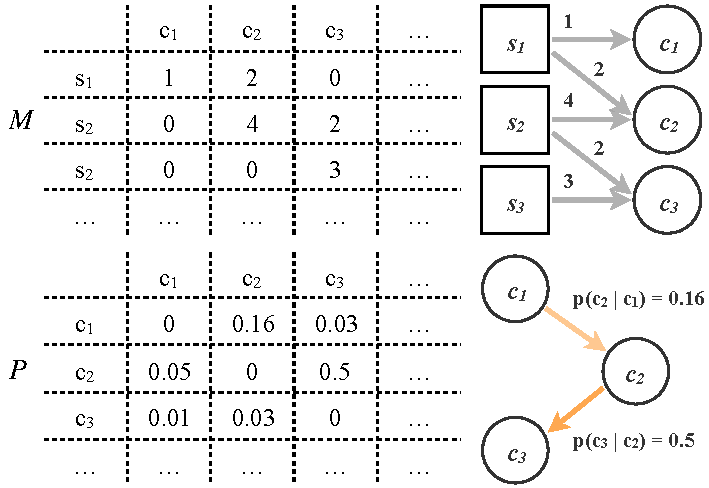
\includegraphics[width=\columnwidth]{Figs/final-simple.pdf}
    \caption{An overview of the projection created from enrollment
      data. Enrollment sequences are tallied and normalized to define
      a conditional probability of taking one course after
      another. Rows $s_i$ describe students, while columns $c_i$
      correspond to course offerings.}
    \label{fig:simple}
\end{figure}

Our first challenge is to build an expressive, yet interpretable model
of course-to-course interactions that results in the graph based
representation of academic pathways. The representation must support
the desired ability to discover student enrollment patterns over time
and enrollment interactions between departments. 

Towards this end, we compile student-to-course enrollment information
into what we will call a course-to-course projection model, a network
that represents courses as nodes and course relationships as weighted
edges. Figure~\ref{fig:simple} illustrates the process. We begin with
a matrix $M$ representing student enrollment in courses over
time. Indeed, we can interpret this matrix $M$ as the adjacency matrix
of a bipartite, labeled graph documenting the interaction of student
nodes with course nodes.  We end with a matrix $P$ that defines a
projection of the courses in $M$, where edge weights signify how
strongly two courses are linked. This projection can be visualized as a network such as the one found in Figure~\ref{fig:overview}, which maps all course interactions in a way that describes the aggregate behavior of student enrollment patterns.

Combined with an existing graph manipulation kit---in our case
\cite{shannon2003cytoscape}---the graph described by $P$ serves as our
target toolkit for university stakeholders. We now show how we endow
the construction process of $P$ with flexibility that can tune the
resulting graph for visualizations that help answer a variety of
questions.

As per the overview above, the first step is to prepare a sequence
matrix. The second involves the calculation of the projection. The
following sections merely formalize the overview.

\subsection{Sequence Matrix Generation}
\label{sec:seq_martix}

{\em Via} receives data in the form of tabular student enrollment
records. The input to the projection algorithm is a matrix $M$ of
shape $(|S|, |C|)$, where $S$ is the set of all students and $C$ is
the set of all courses. A given entry $M_{ij}$ represents the time
when a student $i$ enrolls in some course $j$. For example, an entry
$M_{ij} = 1$ signifies that student $i$ enrolled in course $j$ during
their first academic term, generally quarter or semester. An entry
$M_{ij} = 0$ implies that $i$ never enrolled in $j$. This thus implies
that each row $m_i$ represents the entire course enrollment history of
some student $i$. We generate various forms of matrix $M$ from the raw
enrollment data by filtering on different student attributes. The
nature of the filter depends on the questions being asked. For
example, if we are only interested in those who majored in the Humanities, we would
limit $M$ to this student subset. Another filter one might apply at
this step is year of enrollment, if only that time slice is of
interest. The more filtering is applied to $M$ the faster the
subsequent processing, and visual interaction response.

Our data provides information on each enrollment's time, the enrolling
student's major at the time of enrollment, and the student's final
major. Depending on data availability, filters based on gender, status
as underrepresented minority, or college entrance scores could be
applied as well.

\subsection{Graph Projection}
\label{sec:graph_projection}
Next, given the sequence matrix $M$, we generate the matrix $P$ of
shape $(|C|, |C|)$. This matrix represents the adjacency matrix for a
one-mode projection of the bipartite network specified by matrix
$M$. We weight each edge in $P$ using conditional probabilities that
describe how likely one is to take one course given another
course. Thus, entry $P_{ij}$ represents the conditional probability of
taking course $j$ given that one has taken course $i$. $P$ aggregates
students, losing some information, but gaining the probability of moving from one course to another.

Matrix $P$ is thus a representation of how even non-adjacent course nodes in $M$ interact, based on the nature of student enrollment. We use this matrix $P$ as the basis of all calculations and visualizations. 
 The parameters for the conditional probabilities are fit based on counts determined in the calculation of intermediary matrix $\tilde{P}$ of shape $(|C|, |C|)$. We calculate each entry $\tilde{P}_{ij}$ by accumulating the occurrences of course $i$ taken at some point before course $j$ across all students in set $S$:
\begin{equation}
  \tilde{P}_{ij} = \sum_{s=1}^{|S|} \mathbbm{1}\{M_{si} - M_{sj} \geq 0\}* d(M_{si} - M_{sj})
\end{equation}
where $M_{si} - M_{sj}$ is the academic timestep delta (commonly
measured in semesters, or quarters) between a student $s$'s taking
course $i$ and course $j$. Function $d$ is a second point in the
visualization construction where flexibility is provided. The function
may be chosen to de-emphasize the connection between subsequent
courses.

For example, in an analysis of degree completion we may be interested
in cases when course offerings were taken as closely together as
possible. In contrast, when planning curricula we may wish simply to
learn the probabilities of two courses taken in sequence, even if
several academic terms apart.

Function $d$ may be chosen to be continuous or discrete.  For example,
the following choice attenuates the relationship between two courses
through an exponential decay over enrollment term distance:

\begin{equation}
  \tilde{P}_{ij} = \sum_{s=1}^{|S|} \mathbbm{1}\{M_{si} - M_{sj} \geq 0\}* \lambda^{M_{si} - M_{sj}}
\end{equation}
where, $\lambda$ is a constant that controls decay rate. Intuitively, this type of function gives more weight to close course-pair enrollments than temporally distant course-pair enrollments.

Alternatively, we may choose a function $d$ that tallies a
relationship between two courses only when course $j$ immediately
follows course $i$. In the following example, elapsed time between two
courses beyond one term would sever the relationship:
\begin{equation}
d = \begin{cases} 
      1, & M_{si} - M_{sj} = 1 \\
      0, & M_{si} - M_{sj} > 1 
    \end{cases}
\end{equation}
More elaborate discrete functions could amplify course relationships of
particular time distances.

Using $\tilde{P}$, we calculate the final projection matrix $P$. In some experiments, we set $P = \tilde{P}$, in order to gain access to a raw count projection matrix. In other experiments, we set $P$ to be a matrix of conditional probabilities between courses. In this case, each entry $P_{ij}$ is a conditional probability $p(j|i)$ whose parameters are computed using the following closed form expression:
\begin{equation}
    P_{ij} = p(j|i) = \frac{\tilde{P}_{ij}}{\sum_{s=1}^{|S|}\mathbbm{1}\{M_{si} > 0\}}
\end{equation}
$P_{ij}$ thus represents the proportion of students who take the
course sequence: course $i$ followed by $j$ out of the total number of
students who take course $i$ at any point. One may note that this
bears a resemblance to a Bayesian Network; however, we make the
assumption that the process of transitioning from course node to
course node is Markovian in nature. This eases implementation but
precludes our model from being a true Bayesian Network due to the
emergence of cycles.
%In our domain cycles should be allowed in the model. They describe 

In the following section we describe how we combine the projection
matrix with an existing graph visualization tool. For simplicity we
choose the timestep delta function $d$ to be discrete, although we
will alter the nature of the function for different examples.

